\section{Digital options}\lesson{14}{09/04/2020}
Digital options are related to a specific type of European options for which the payoff is either some fixed monetary amount or nothing at all:
\begin{equation}
    \pay_T = \mathds{1}_{S_T\ge K}.
\end{equation}

\subsection{Pricing}
For pricing we could adapt the risk neutral methodology, but there is a much simpler way. In fact, we can write the call payoff as:
\begin{align}
    (S_T-K)^+ &= (S_T-K)\mathds{1}_{S_T\ge K} = S_T\mathds{1}_{S_T\ge K} - K\mathds{1}_{S_T\ge K}.
\end{align}
So, the price of the digital option payoff is:
\begin{align}
    \notag price^{DIG}_t &= e^{-r(T-t)}\expect_t[\mathds{1}_{S_T\ge K}] \\
    &=
    \notag e^{-r(T-t)}\Qmeas_t(S_T\ge K) \\
    &=
    e^{-r(T-t)}\Phi(d_2),
\end{align}
where $\Qmeas$ is the conditional risk neutral probability. We only have to compute the gaussian CDF. The problems appear when we consider the hedging: we saw that in the call option the payoff is continuous (it is the solution of a PDE) and differentiable. Here the payoff is not continuous, so we expect additional irregularities in the Greeks.

\subsection{Hedging}
Recall that
\begin{equation*}
    \Phi(d_2) = \int^{d_2}_{-\infty} \dfrac{e^{-\frac{x^2}{2}}}{\sqrt{2\pi}}\,dx \qquad\Rightarrow\qquad \pdv{\Phi(d_2)}{S} = \dfrac{e^{-\frac{d_2^2}{2}}}{\sqrt{2\pi}}\dfrac{1}{S\sigma\sqrt{T-t}},
\end{equation*}
so the delta is
\begin{equation}
    \Delta^{DIG}_t = \dfrac{e^{-r(T-t)}e^{-\frac{d_2^2}{2}}}{\sqrt{2\pi}S\sigma\sqrt{T-t}}
\end{equation}
and in this case its shape is like a Dirac delta.
\begin{figure}[htp]
    \centering
    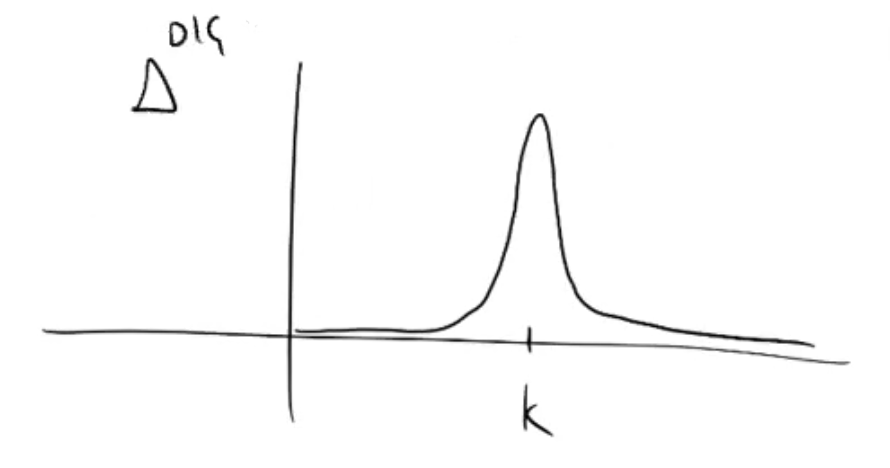
\includegraphics[scale=0.3]{fig/tmp/fig24.png}
    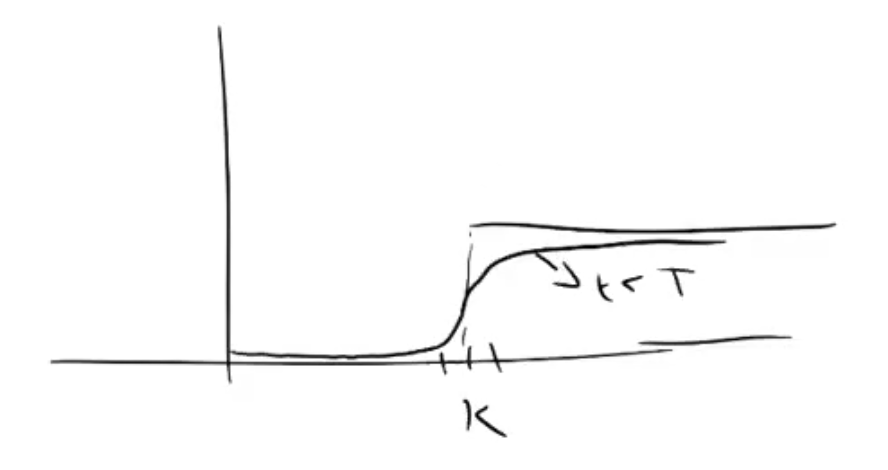
\includegraphics[scale=0.3]{fig/tmp/fig25.png}
    \caption{(a) Delta and (b) pricing function for the digital options.}
    \label{fig:digdelta}
\end{figure}
\newline With such a delta, if the underlying fluctuates in a small interval around the strike, it is impossible to hedge a digital option. In fact, the price function is such that it is impossible to buy or sell without incurring in a huge risk (in correspondence of the unitary jump). \\
Unfortunately, the traders' portfolios are typically full of digital options because they think in a myopic way: three years and three years plus a week are almost the same. So, if they have to match some conditions in a horizon of three years, they look in the market for some products with maturity quite close to the one they have to hedge. But as time goes by the maturity approaches and if for example we hedge with an option which maturity is a bit shorter there will be a small additional increment of maturity (one week) in which we are uncovered (or in some other cases overcovered, i.e. we are over-hedging). The way traders hedge digital options is like a proxy, in the sense that instead of considering the true payoff of the option (the step function) they consider a combination of different options. For example, they consider a long call with strike $K_1$ and a short call with strike $K_2$ (Figure \ref{fig:dighedge}). This combination is called \emph{bull spread} (we have limited profits but limited losses).
\begin{figure}[htp]
    \centering
    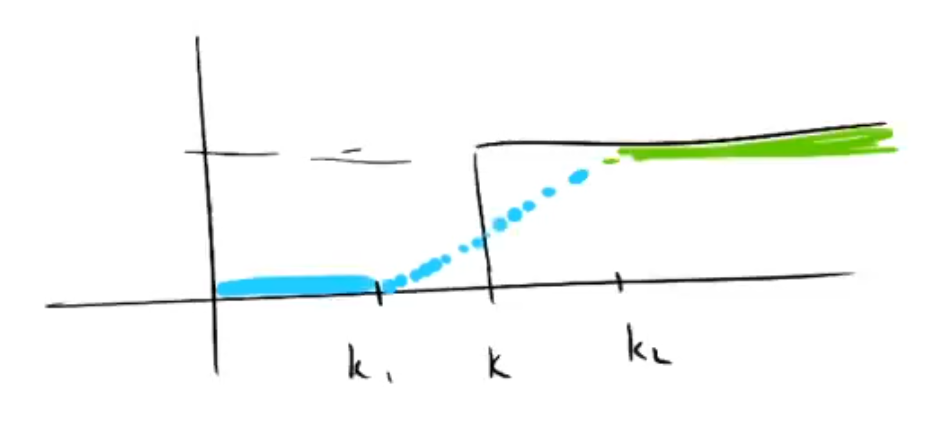
\includegraphics[scale=0.3]{fig/tmp/fig26.png}
    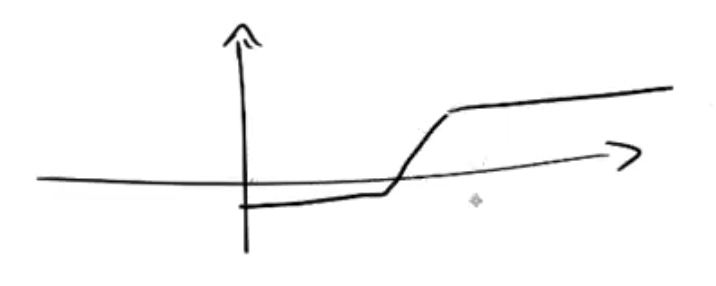
\includegraphics[scale=0.3]{fig/tmp/fig27.png}
    \caption{Bull spread.}
    \label{fig:dighedge}
\end{figure}
\newline Let's consider the gamma:
\begin{equation}
    \Gamma^{DIG} = \pdv{\Delta^{DIG}}{S}
\end{equation}
The explicit expression is not very interesting, the important thing is that it can be both positive or negative. If it is negative there is the possibility to incur in very heavy losses for large fluctuations of the underlying. This is an example of \emph{exotic options}, because it is very difficult to hedge and it has a potential negative gamma.
\begin{example}{}{}{}
    Consider the following payoff:
    \begin{equation}
        \pay_T = \begin{cases}
        -c_1 & S_T \in [0,K_1) \\
        S_T - K_1 - c_1 & S_T \in [K_1,K_2) \\
        K_3 - S_T - c_2 & S_T \in [K_2,K_3) \\
        -c_2 & S_T \ge K_3
        \end{cases}
    \end{equation}
    where $0<c_1<c_2$ and $0<K_1<K_2<K_3$.
    \begin{enumerate}
        \item How can we price a product which leads to this payoff?
        \item Which is the form of delta and gamma?
        \item Show how the price changes for an upward shift of the volatility $\sigma_1\to\sigma_2>\sigma_1$.
    \end{enumerate}
    \textbf{Solution.} 1. First, let's visualize the payoff function.
    \begin{center}
        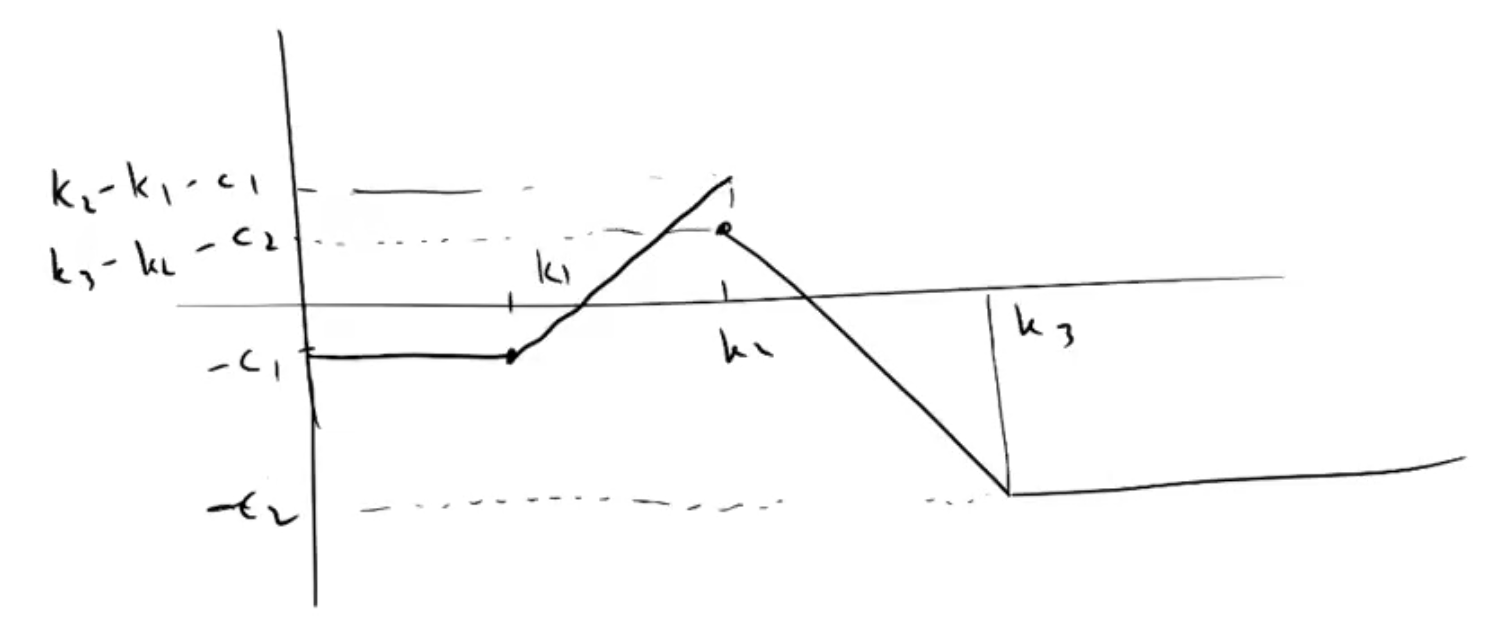
\includegraphics[scale=0.3]{fig/tmp/fig28.png}
    \end{center}
    In principle, we can always write the price as the discounted value of the risk neutral expectation of the payoff:
    \begin{align}
        \notag price_t(\pay_T) &= e^{-r(T-t)}\expect_t[\pay_T] \\
        &=
        e^{-r(T-t)}\left(\int_{-\infty}^{K_1}\dots+\int_{K_1}^{K_2}\dots+\int_{K_2}^{K_3}\dots+\int_{K_3}^{+\infty}\dots\right)
    \end{align}
    However, we would like to avoid brute force integration. Instead, we would like to write this expression in terms of some building blocks we already know how to price. We can start from the left or from the right. If we start from the left, the idea is to start with some product and add something else such that what is on the left remains unchanged and in case of need we can change what is in the right. But we know something that leaves the left unchanged: the call option. In fact, when the underlying is smaller than the strike, the call option has no effect. If we start from the right, the opposite holds and we can use put options.\\
    Let's start from the left. The payoff decomposition is the following:
    \begin{itemize}
        \item The payoff starts from $-c_1$ and it is constant till $K_1$. In order to have a straight line with slope $+1$ we consider a long position in a call option with strike $K_1$:
        \begin{equation*}
            \pay_T = -c_1 + (S_T+K_1)^+ +\dots
        \end{equation*}
        \item Now, in order to change the slope from $-1$ to 1 we take two short positions in a call with strike $K_2$:
        \begin{equation*}
            \pay_T = -c_1 + (S_T-K_1)^+ - 2(S_T-K_2)^+ + \dots
        \end{equation*}
        and in order to have the discontinuity in $K_2$ we translate downward the payoff by taking a number of short positions in a digital option equal to the size of the step:
        \begin{align*}
            \pay_T &= -c_1 + (S_T-K_1)^+ - 2(S_T-K_2)^+ - \\
            &\qquad
            -(K_2-K_1-c_1-(K_3-K_2-c_2))\mathds{1}_{S_T\ge K_2} + \dots
        \end{align*}
        \item Now at $K_3$ we change the slope from $-1$ to 0 by taking a long position in a call with strike $K_3$:
        \begin{align}
            \notag \pay_T &= -c_1 + (S_T-K_1)^+ - 2(S_T-K_2)^+ - \\
            &\qquad
            -(K_2-K_1-c_1-(K_3-K_2-c_2))\mathds{1}_{S_T\ge K_2} + (S_T-K_3)^+.
        \end{align}
    \end{itemize}
    The corresponding price of this payoff is:
    \begin{align} %34:00
        \notag price_t(\pay_T) &= -c_1e^{-r(T-t)} + S_t\Phi(d_1^{K_1}) - e^{-r(T-t)}K_1\Phi(d_2^{K_1}) - \\
        &\qquad
        \notag - 2(S_t\Phi(d_1^{K_2})-e^{-r(T-t)}K_2\Phi(d_2^{K_2})) - \\
        &\qquad
        \notag - (2K_2-K_1-K_3-c_1+c_2)e^{-r(T-t)}\Phi(d_2^{K_2}) + \\
        &\qquad
        + S_t\Phi(d_1^{K_3}) - e^{-r(T-t)}K_3\Phi(d_2^{K_3}),
    \end{align}
    where
    \begin{equation}
        d_1^{K_i} = \dfrac{\ln\frac{S}{K_i}+\left(r+\frac{\sigma^2}{2}\right)(T-t)}{\sigma\sqrt{T-t}}, \qquad i = 1,2,3.
    \end{equation}
    2. The delta is given by the sum of the building blocks' deltas:
    \begin{align}
        \Delta_t = 0 + \Phi(d_1^{K_1}) - 2\Phi(d_1^{K_2}) - \Delta^{DIG, K_2} + \Phi(d_1^{K_3})
    \end{align}
    and the gamma is
    \begin{equation}
        \Gamma_t = 0 + \dfrac{1}{S_t\sigma\sqrt{T-t}}\dfrac{e^{-\frac{d_1^{K_1}}{2}}}{\sqrt{2\pi}} - 2\dfrac{1}{S\sigma\sqrt{T-t}}\dfrac{e^{-\frac{d_1^{K_2}}{2}}}{\sqrt{2\pi}} - \Gamma^{DIG,K_2} + \dfrac{1}{S_t\sigma\sqrt{T-t}}\dfrac{e^{-\frac{d_1^{K_3}}{2}}}{\sqrt{2\pi}}.
    \end{equation}
    3. If the volatility is $\sigma_2>\sigma_1$ the pricing function will be smoother. %fine parte 1
    \begin{center}
        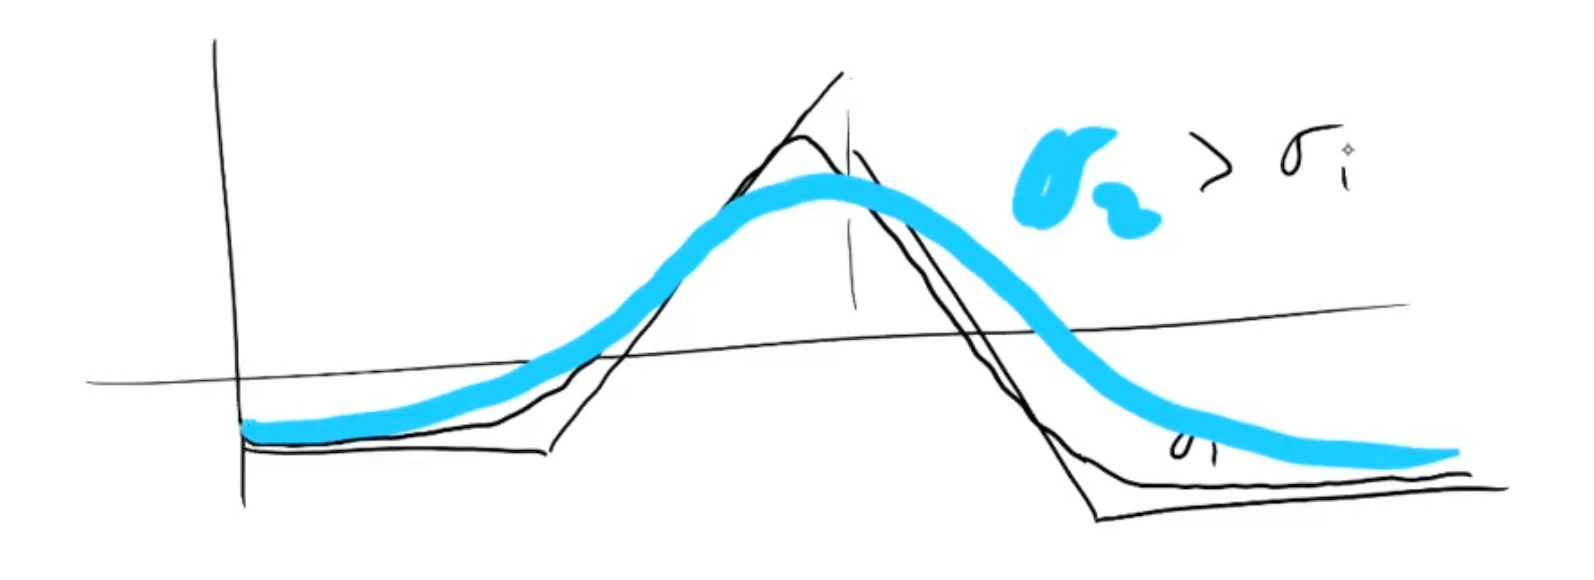
\includegraphics[scale=0.3]{fig/tmp/fig29.png}
    \end{center}
\end{example}

\section{Black \& Scholes model with continuous dividends}\label{B&Swithdividends}
In this section we consider the case when dividends are paid out continuously in time. As usual $S_t$ denotes the price of the stock at time $t$, and we denote the cumulative dividends over the interval $[0,t]$ as
\begin{equation}
    D(t) = \int^t_0 \Tilde{\delta}_s \, \dd s
\end{equation}{}
where $\Tilde{\delta}$ is the rate of dividends. Put in differential form, this means that over the infinitesimal interval $(t, t + \dd t]$ the holder of the stock receives the amount $\dd D(t) = D(t + \dd t) - D(t)$.\\
The starting point is the B\&S formula:
\begin{equation}
    \dfrac{\dd S}{S} = \mu\dd t + \sigma \dd W^{\Pmeas}
\end{equation}
where $\Pmeas$ is the historical probability measure. We still don't know which is the risk neutral probability measure because here the price of the asset changes differently according to the fact that some dividends are delivered or not. So, in order to find the risk neutral measure $\Qmeas$ we have to start from the beginning. We define our portfolio as
\begin{equation}
    V_t = h_t\cdot S_t, \qquad S_t = \binom{S_t}{e^{rt}}.
\end{equation}
The old portfolio (before dividends) has value $h(t-\Delta t)S(t)$. Suppose that at time $t$ there is a delivery of some dividends, such that we get $h(t-\Delta t)(D(t)-D(t-\Delta t))$. The budget equation is given by:
\begin{equation}
    h(t-\Delta t)S(t) + h(t-\Delta t)(D(t)-D(t-\Delta t)) = h(t)S(t) + c(t)\Delta t.
\end{equation}
If we add and subtract $S(t-\Delta t)\Delta h(t)$ we end up with:
\begin{align}
    \notag\dd V_t &= h(t)\dd S_t + h(t)\dd D_t - c(t)\dd t \\
    &=
    h(t)(\dd S_t + \dd D_t) - c(t)\dd t.
\end{align}
In the presence of dividends, the self financing condition involves a \emph{gain process}, because in addition to the price we get something more, i.e. the dividends (which can be seen as an incoming salary). Since $\dd D(t) = D(t + \dd t) - D(t)$ is a forward increment we can use Itô's formula. Now, under the measure $\Qmeas$, we want the discounted asset with the additional presence of the value of the future streams of dividends
\begin{equation}
    S_te^{-rt} + \int_0^t e^{-rs}\dd D_s
\end{equation}
to be a martingale. This process is called \emph{normalized gain process}. \\
Now we look for the pricing PDE. Starting from the dynamics of our portfolio
\begin{equation}
    \begin{cases}
    \dd V = h \dd S + h \dd D + 0 \\
    V_T = \pay_T = F(S_T,T),
    \end{cases}
\end{equation}
where the 0 means no consumption, we have
\begin{equation}\label{hsd}
    h_t \dd S_t + h_t \dd D_t = \pdv{F}{t}\dd t + \pdv{F}{S}\dd S + \dfrac{1}{2}\sigma^2S_t^2\pdv[2]{F}{S}\dd t.
\end{equation}
Recall that
\begin{equation}
    h = \binom{\alpha}{\beta}, \qquad S_t = \binom{S}{e^{rt}}, \qquad D = \binom{\int^t_0\Tilde{\delta}_s\,\dd s}{0},
\end{equation}
where the second element of $D$ is zero because there are no dividends in the riskless asset. Substituting in \eqref{hsd} we get:
\begin{align}\label{ll}
    \notag\hlc{mypink}{\alpha S(\mu\dd t + \sigma\dd W^{\Pmeas})}+\beta re^{rt}\dd t + \alpha\Tilde{\delta}_t\dd t =\, &\pdv{F}{t}\dd t + \hlc{mypink}{\pdv{F}{S}S(\mu\dd t + \sigma\dd W^{\Pmeas})} + \\
    &+ \dfrac{1}{2}\sigma^2S_t^2\pdv[2]{F}{S}\dd t.
\end{align}
Comparing the pink boxes, we see that, even in presence of dividends, $\alpha$ is still given by
\begin{equation}\label{a}
    \alpha = \pdv{F}{S} = \Delta_t.
\end{equation}
Substituting \eqref{a} in \eqref{ll}, the two pink terms cancel out and we get the following PDE:
\begin{equation}
    \pdv{F}{t}\dd t + rS\pdv{F}{S} + \dfrac{1}{2}\sigma^2S_t^2\pdv[2]{F}{S} - \Tilde{\delta}\pdv{F}{S} - rF = 0.
\end{equation}
Financially speaking, it is not reasonable that $\Tilde{\delta}$ is constant, because the rate of dividends should depend on the value of the asset. The typical assumption is that $\tilde{\delta}$ is given by a constant $q$ times the value of the asset at time $t$:
\begin{equation}
    \Tilde{\delta} = qS_t.
\end{equation}
In this case we speak about \emph{proportional dividends}, and the corresponding PDE reads
\begin{equation}
    \begin{cases}
    \pdv{F}{t}\dd t + (r-q)S\pdv{F}{S} + \dfrac{1}{2}\sigma^2S_t^2\pdv[2]{F}{S} - rF = 0 \\
    F(S_T,T) = \pay_T.
    \end{cases}
\end{equation}
Now we apply the Feynman-Kac methodology in order to say that if $F$ is a solution of this PDE then there exist a probability space and a probability measure $\Qmeas^q$ under which we can define the B\&S equation
\begin{equation}\label{gheogjegojrgi}
    \dfrac{\dd S}{S} = (r-q)\dd t + \sigma \dd W^{\Qmeas^q}.
\end{equation}
Such solution of the PDE can be written as
\begin{equation}
    F(S_t,t) = e^{-r(T-t)}\mathbb{E}^{\Qmeas^q}_t[\pay_T].
\end{equation}
Recall that $S_t$ is the solution of the geometric Brownian motion equation \eqref{gheogjegojrgi}. In presence of dividends we have:
\begin{align}
    S_t &= S_0e^{\left(r-q-\frac{1}{2}\sigma^2\right)T+\sigma W_T^{\Qmeas^q}} \\
    &=
    (S_0e^{-qT})e^{\left(r-\frac{1}{2}\sigma^2\right)T+\sigma W_T^{\Qmeas^q}}.
\end{align}
Notice also that, since we can write $(S_0e^{-qT})$ as a new initial value, we have that
\begin{equation}
    F_q(S_t,t) = F_0(S_te^{-q( T-t)}).
\end{equation}
Now we are ready to write the Black \& Scholes formula in presence of dividends:
\begin{equation}
    price^{\call}(t,T,S_t,K,\sigma,r,q) = S_te^{-q( T-t)}\Phi(d_1)-Ke^{-r(T-t)}\Phi(d_2)
\end{equation}
with
\begin{equation}
    d_1 = \dfrac{\ln\frac{S_te^{-q(T-t)}}{K}+\left(r+\frac{1}{2}\sigma^2\right)(T-t)}{\sigma\sqrt{T-t}} = \dfrac{\ln\frac{S_t}{K}+\left(r-q+\frac{1}{2}\sigma^2\right)(T-t)}{\sigma\sqrt{T-t}},
\end{equation}
\begin{equation}
    d_2 = d_1 - \sigma\sqrt{T-t}.
\end{equation}
Using the put-call parity we immediately get the price of a put option.
